\documentclass[../document.tex]{subfiles}
\begin{document}\label{ssec:time}
	
We first present execution time measurements for each benchmark, starting with the Cyclic Redundancy Check {\tt crc} benchmark which represents the Combinational Logic dwarf.

\newcommand{\plotwidth}{0.24\textwidth}
%\begin{figure*}[t]
%	\centering
%	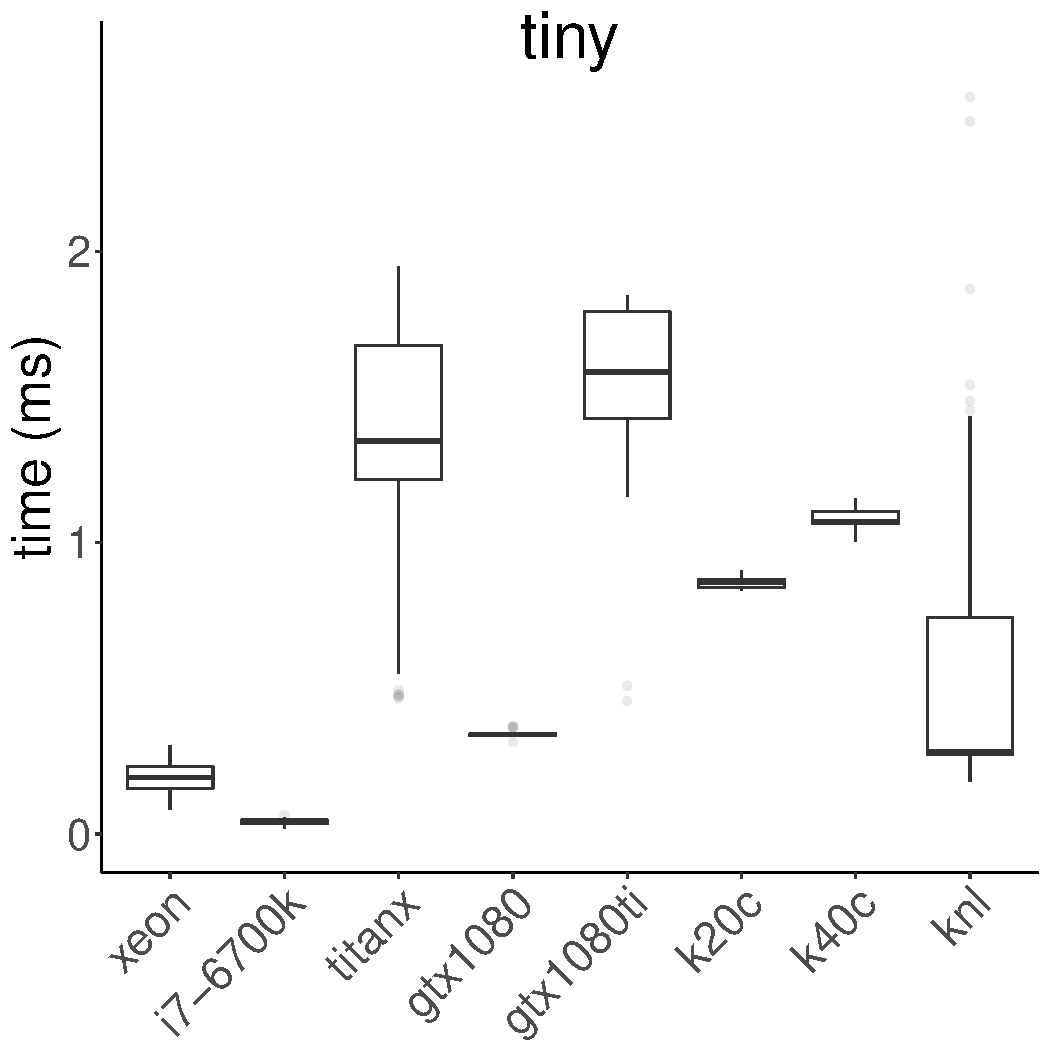
\includegraphics[width=\plotwidth]{figures/time-results/generate_crc_tiny_boxplot_knl-1}
%	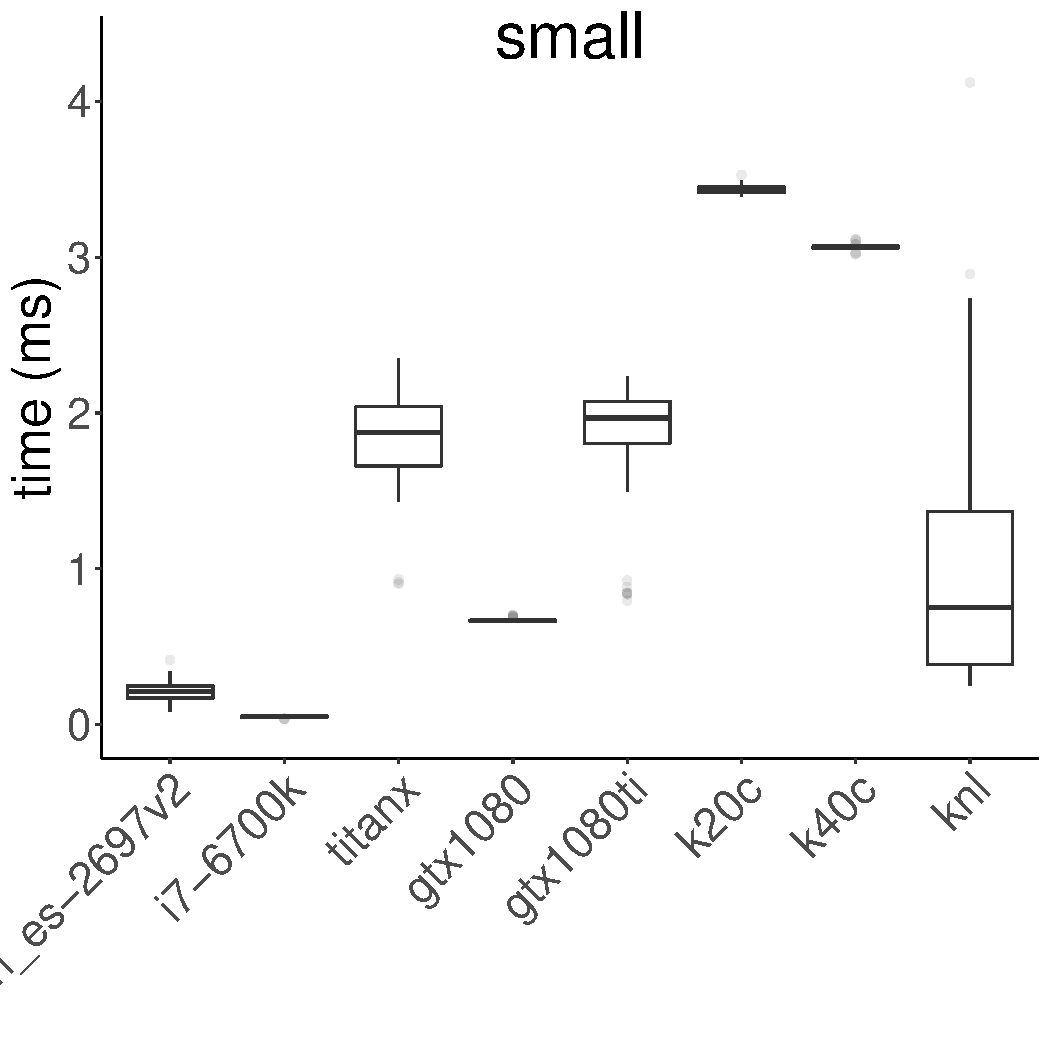
\includegraphics[width=\plotwidth]{figures/time-results/generate_crc_small_boxplot_knl-1}
%	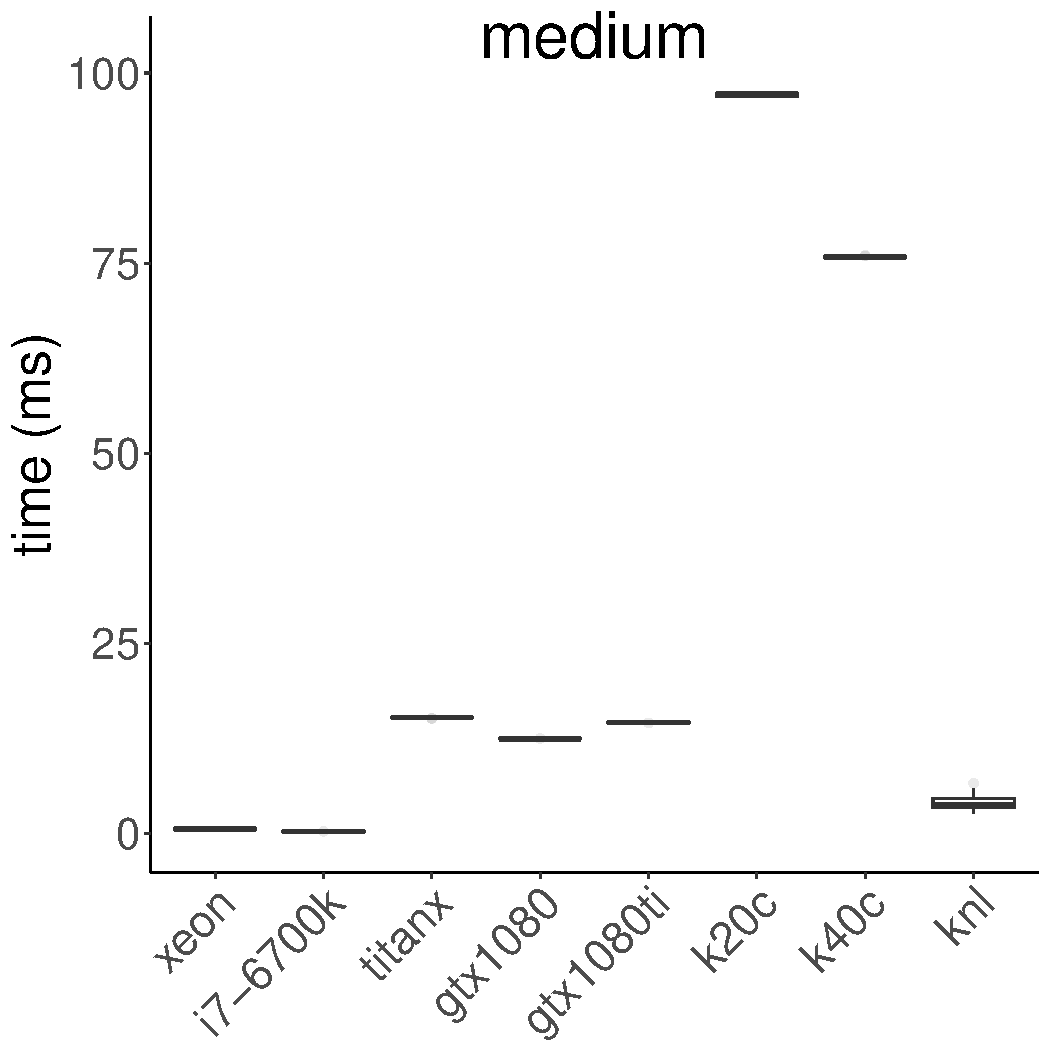
\includegraphics[width=\plotwidth]{figures/time-results/generate_crc_medium_boxplot_knl-1}
%	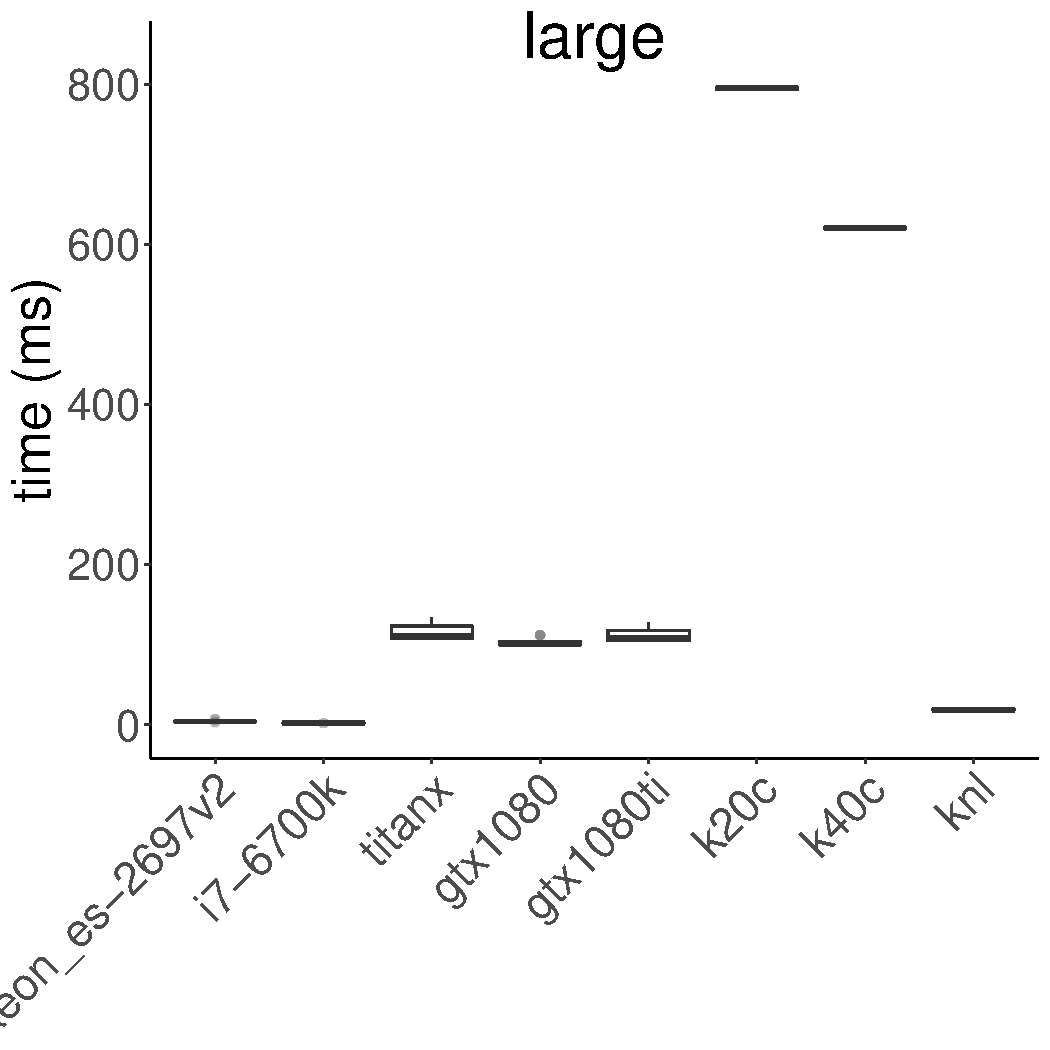
\includegraphics[width=\plotwidth]{figures/time-results/generate_crc_large_boxplot_knl-1}
%	\caption{Kernel execution times for the {\bf crc} benchmark on different hardware platforms, including KNL}
%	\label{fig:time-crc}
%\end{figure*}

\begin{figure*}[t]
	\centering
	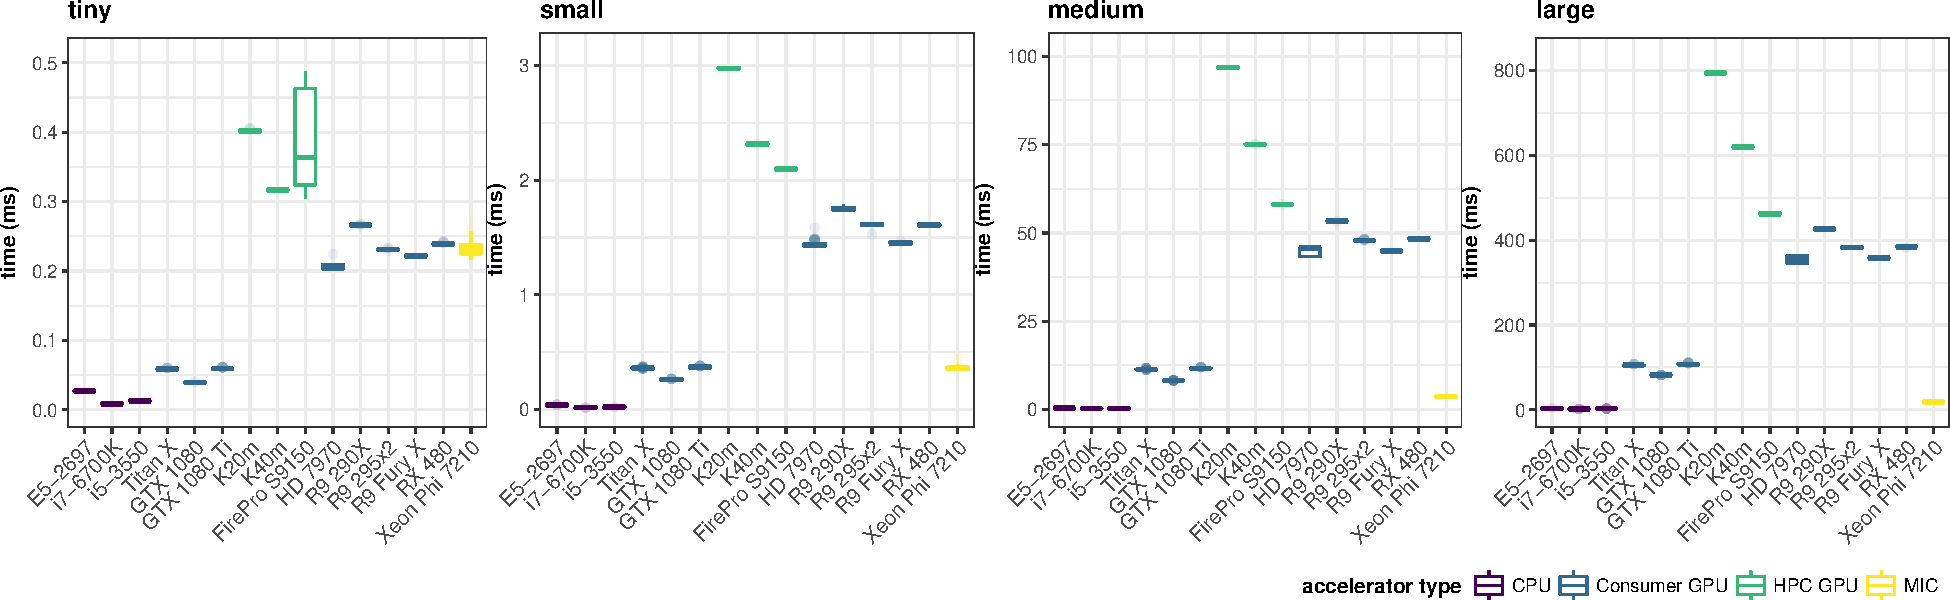
\includegraphics[width=\textwidth,keepaspectratio]{figures/new-time-results/generate_crc_row_bandwplot}
	\caption{Kernel execution times for the {\bf crc} benchmark on different hardware platforms}
	\label{fig:time-crc}
\end{figure*}


Figure~\ref{fig:time-crc} shows the execution times for the {\tt crc} benchmark over 50 iterations on each of the target architectures, including the KNL.
%Each result is the combined execution time of a kernel for a given iteration.
%For instance, s
The results are colored according to accelerator type: purple for CPU devices, blue for consumer GPUs, green for HPC GPUs, and yellow for the KNL MIC.
Execution times for {\tt crc} are lowest on CPU-type architectures, probably due to the low floating-point intensity of the CRC computation~\cite[Ch. 6]{joshi2016thesis}.
Excluding {\tt crc}, all the other benchmarks perform best on GPU type accelerators; furthermore, the performance on the KNL is poor due to the lack of support for wide vector registers in Intel's OpenCL SDK.
We therefore omit results for KNL for the remaining benchmarks.

\todo{We could examine the kiviat diagrams to see if they have high memory address entropy -- or high memory overhead which contributes to the why some benchmarks see a wide variation while others experience only a little, is this the major cause in variation?}
\todo{What are the major motivations for including this results section? We should conclude with these motivations and what has been shown accordingly}

Figures~\ref{fig:time} and~\ref{fig:time2} shows the distribution of kernel execution times for the remaining benchmarks.
Some benchmarks execute more than one kernel on the accelerator device; the reported iteration time is the sum of all compute time spent on the accelerator for all kernels.
Each benchmark corresponds to a particular dwarf: 
Figure~\ref{fig:time}a ({\tt kmeans}) represents the MapReduce dwarf,
Figure~\ref{fig:time}b ({\tt lud}) represents the Dense Linear Algebra dwarf,
Figure~\ref{fig:time}c ({\tt csr}) represents Sparse Linear Algebra, 
Figure~\ref{fig:time}d ({\tt dwt}) and Figure~\ref{fig:time}e ({\tt fft}) represent Spectral Methods,
Figure~\ref{fig:time2}a ({\tt srad}) represents the Structured Grid dwarf and Figure~\ref{fig:time2}b ({\tt nw}) represents Dynamic Programming.

Finally, Figure~\ref{fig:time3} presents results for the three applications with restricted problem sizes and only one problem size is shown.
The N-body Methods dwarf is represented by ({\tt gem}) and the results are shown in Figure~\ref{fig:time3}a, the Backtrack \& Branch and Bound dwarf is represented by the ({\tt nqueens}) application in Figure~\ref{fig:time3}b and ({\tt hmm}) results in Figure~\ref{fig:time3}c represent the Graphical Models dwarf.


\begin{figure*}
    \centering
    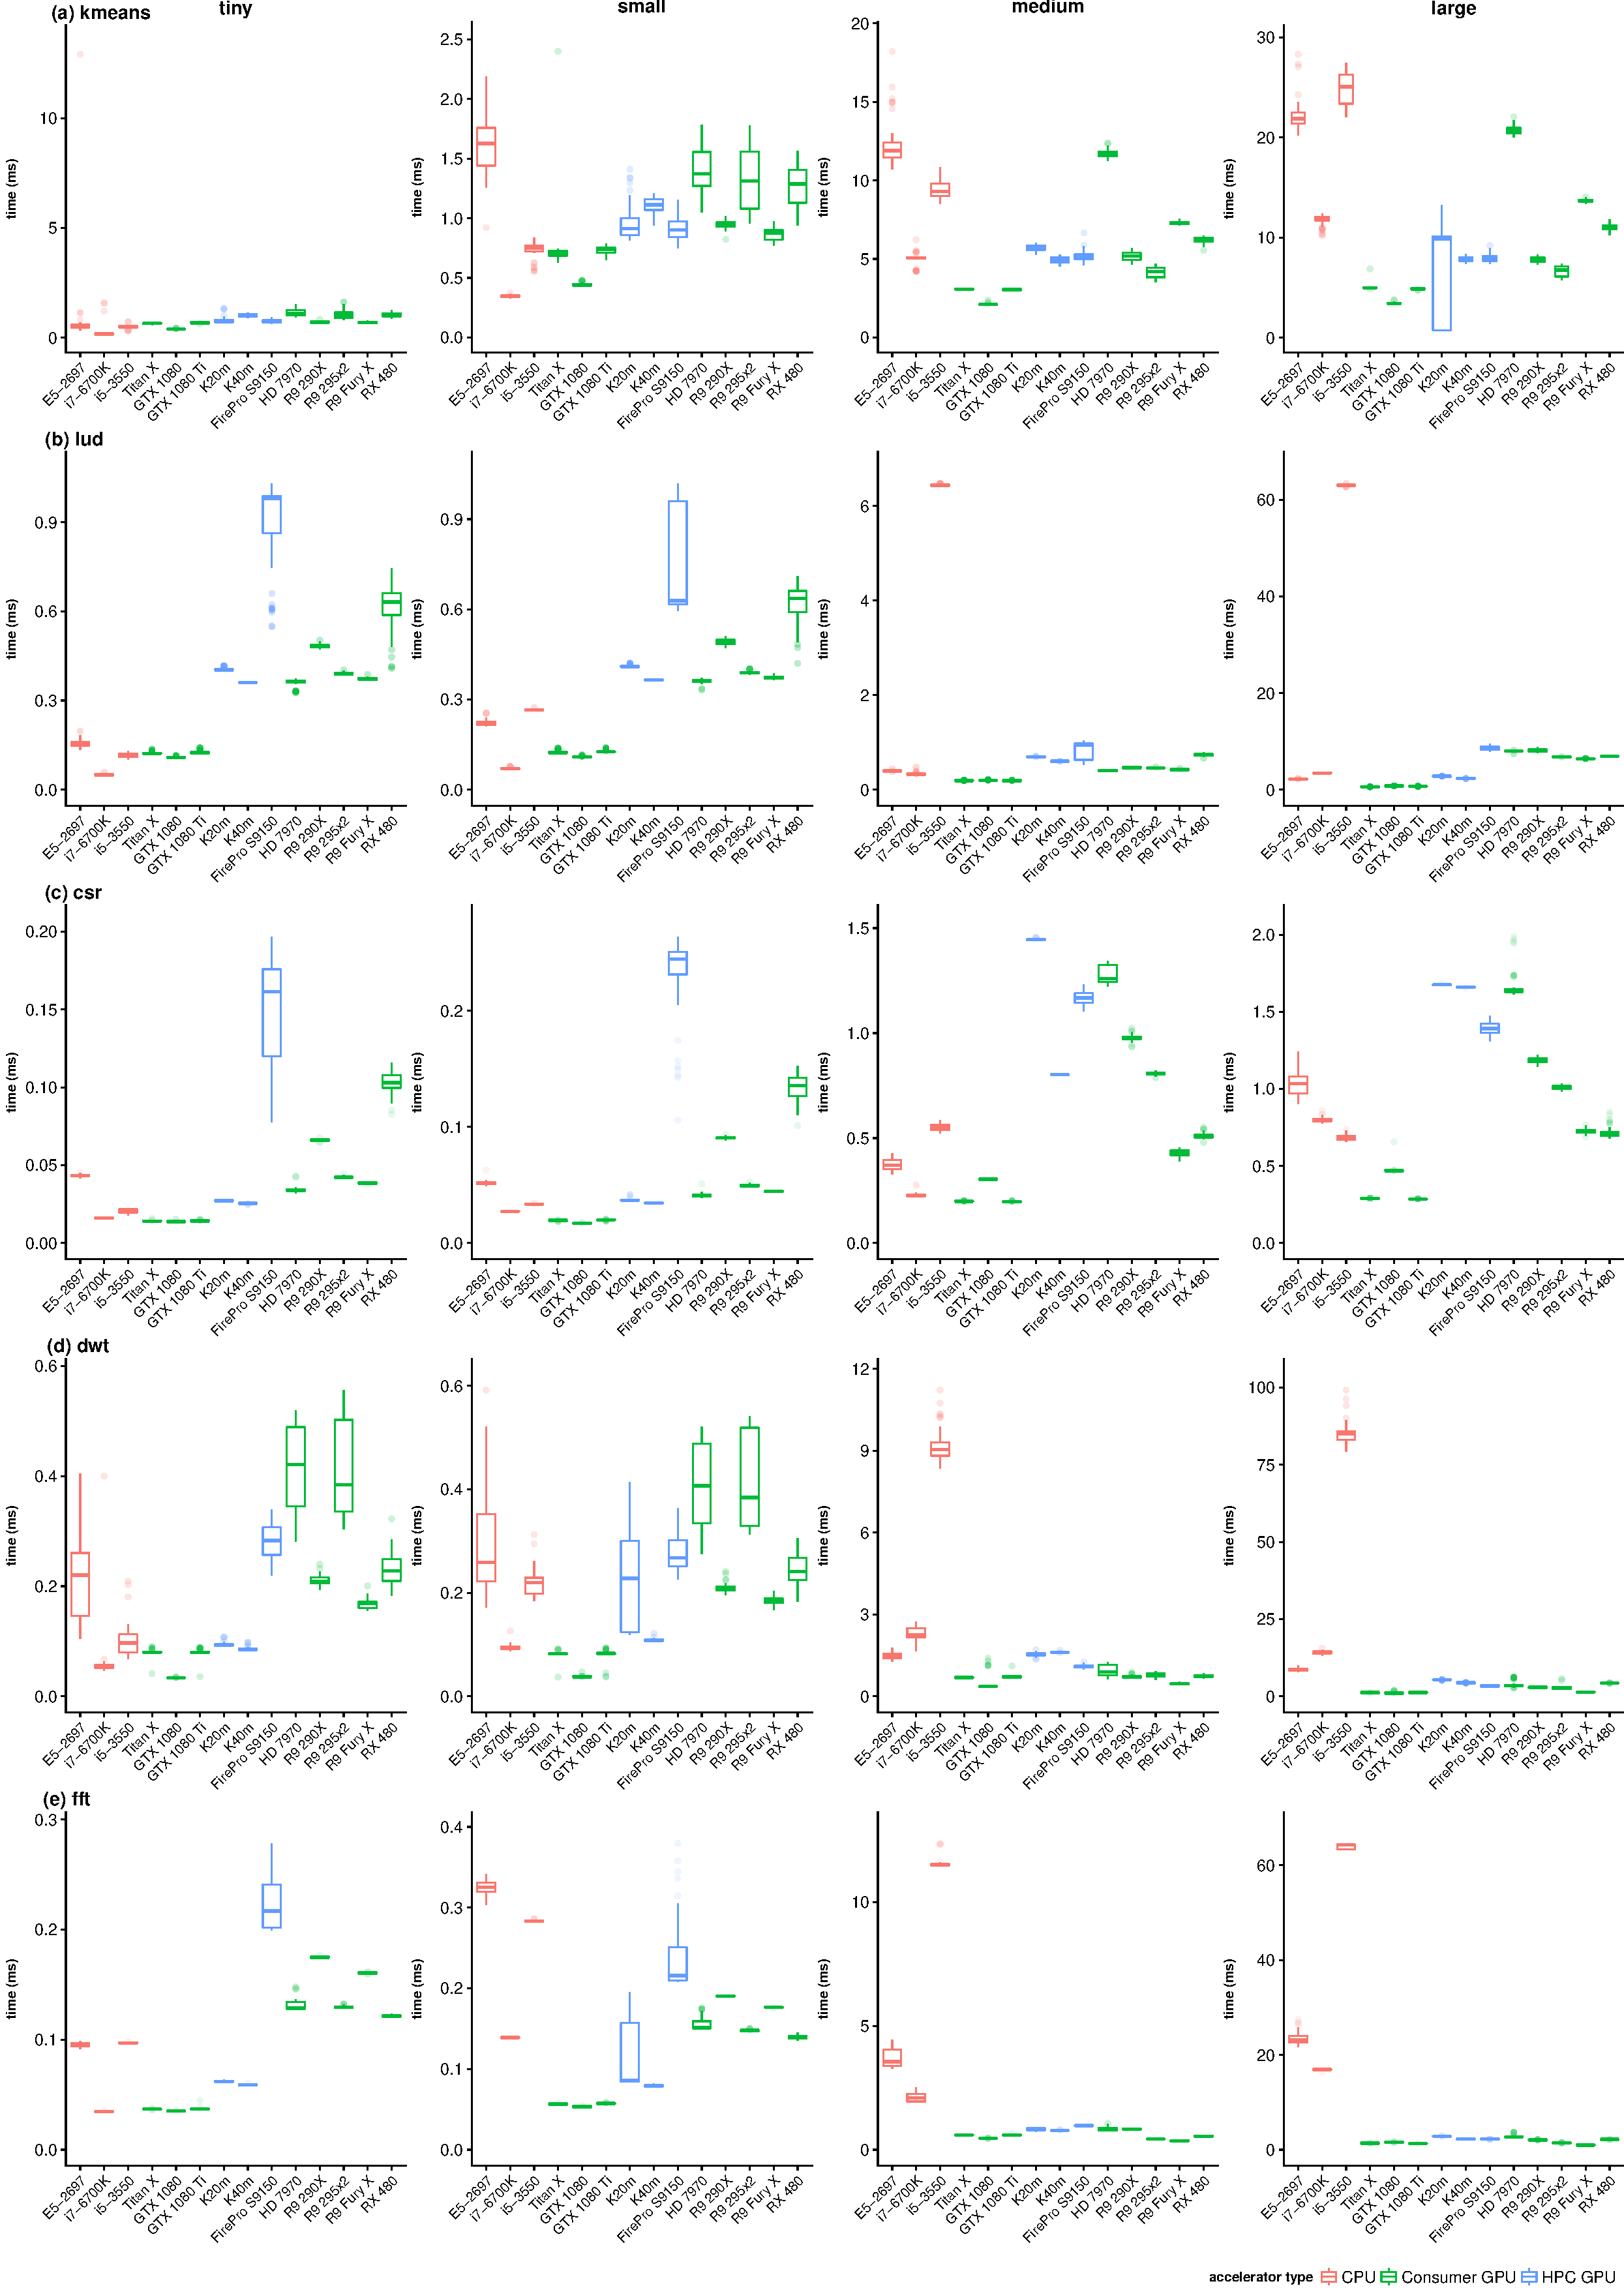
\includegraphics[height=0.96\textheight,width=\textwidth,keepaspectratio]{figures/new-time-results/generate_main_4x5_bandwplot}
    \caption{Benchmark kernel execution times on different hardware platforms}
    \label{fig:time}
\end{figure*}

\begin{figure*}[t]
    \centering
    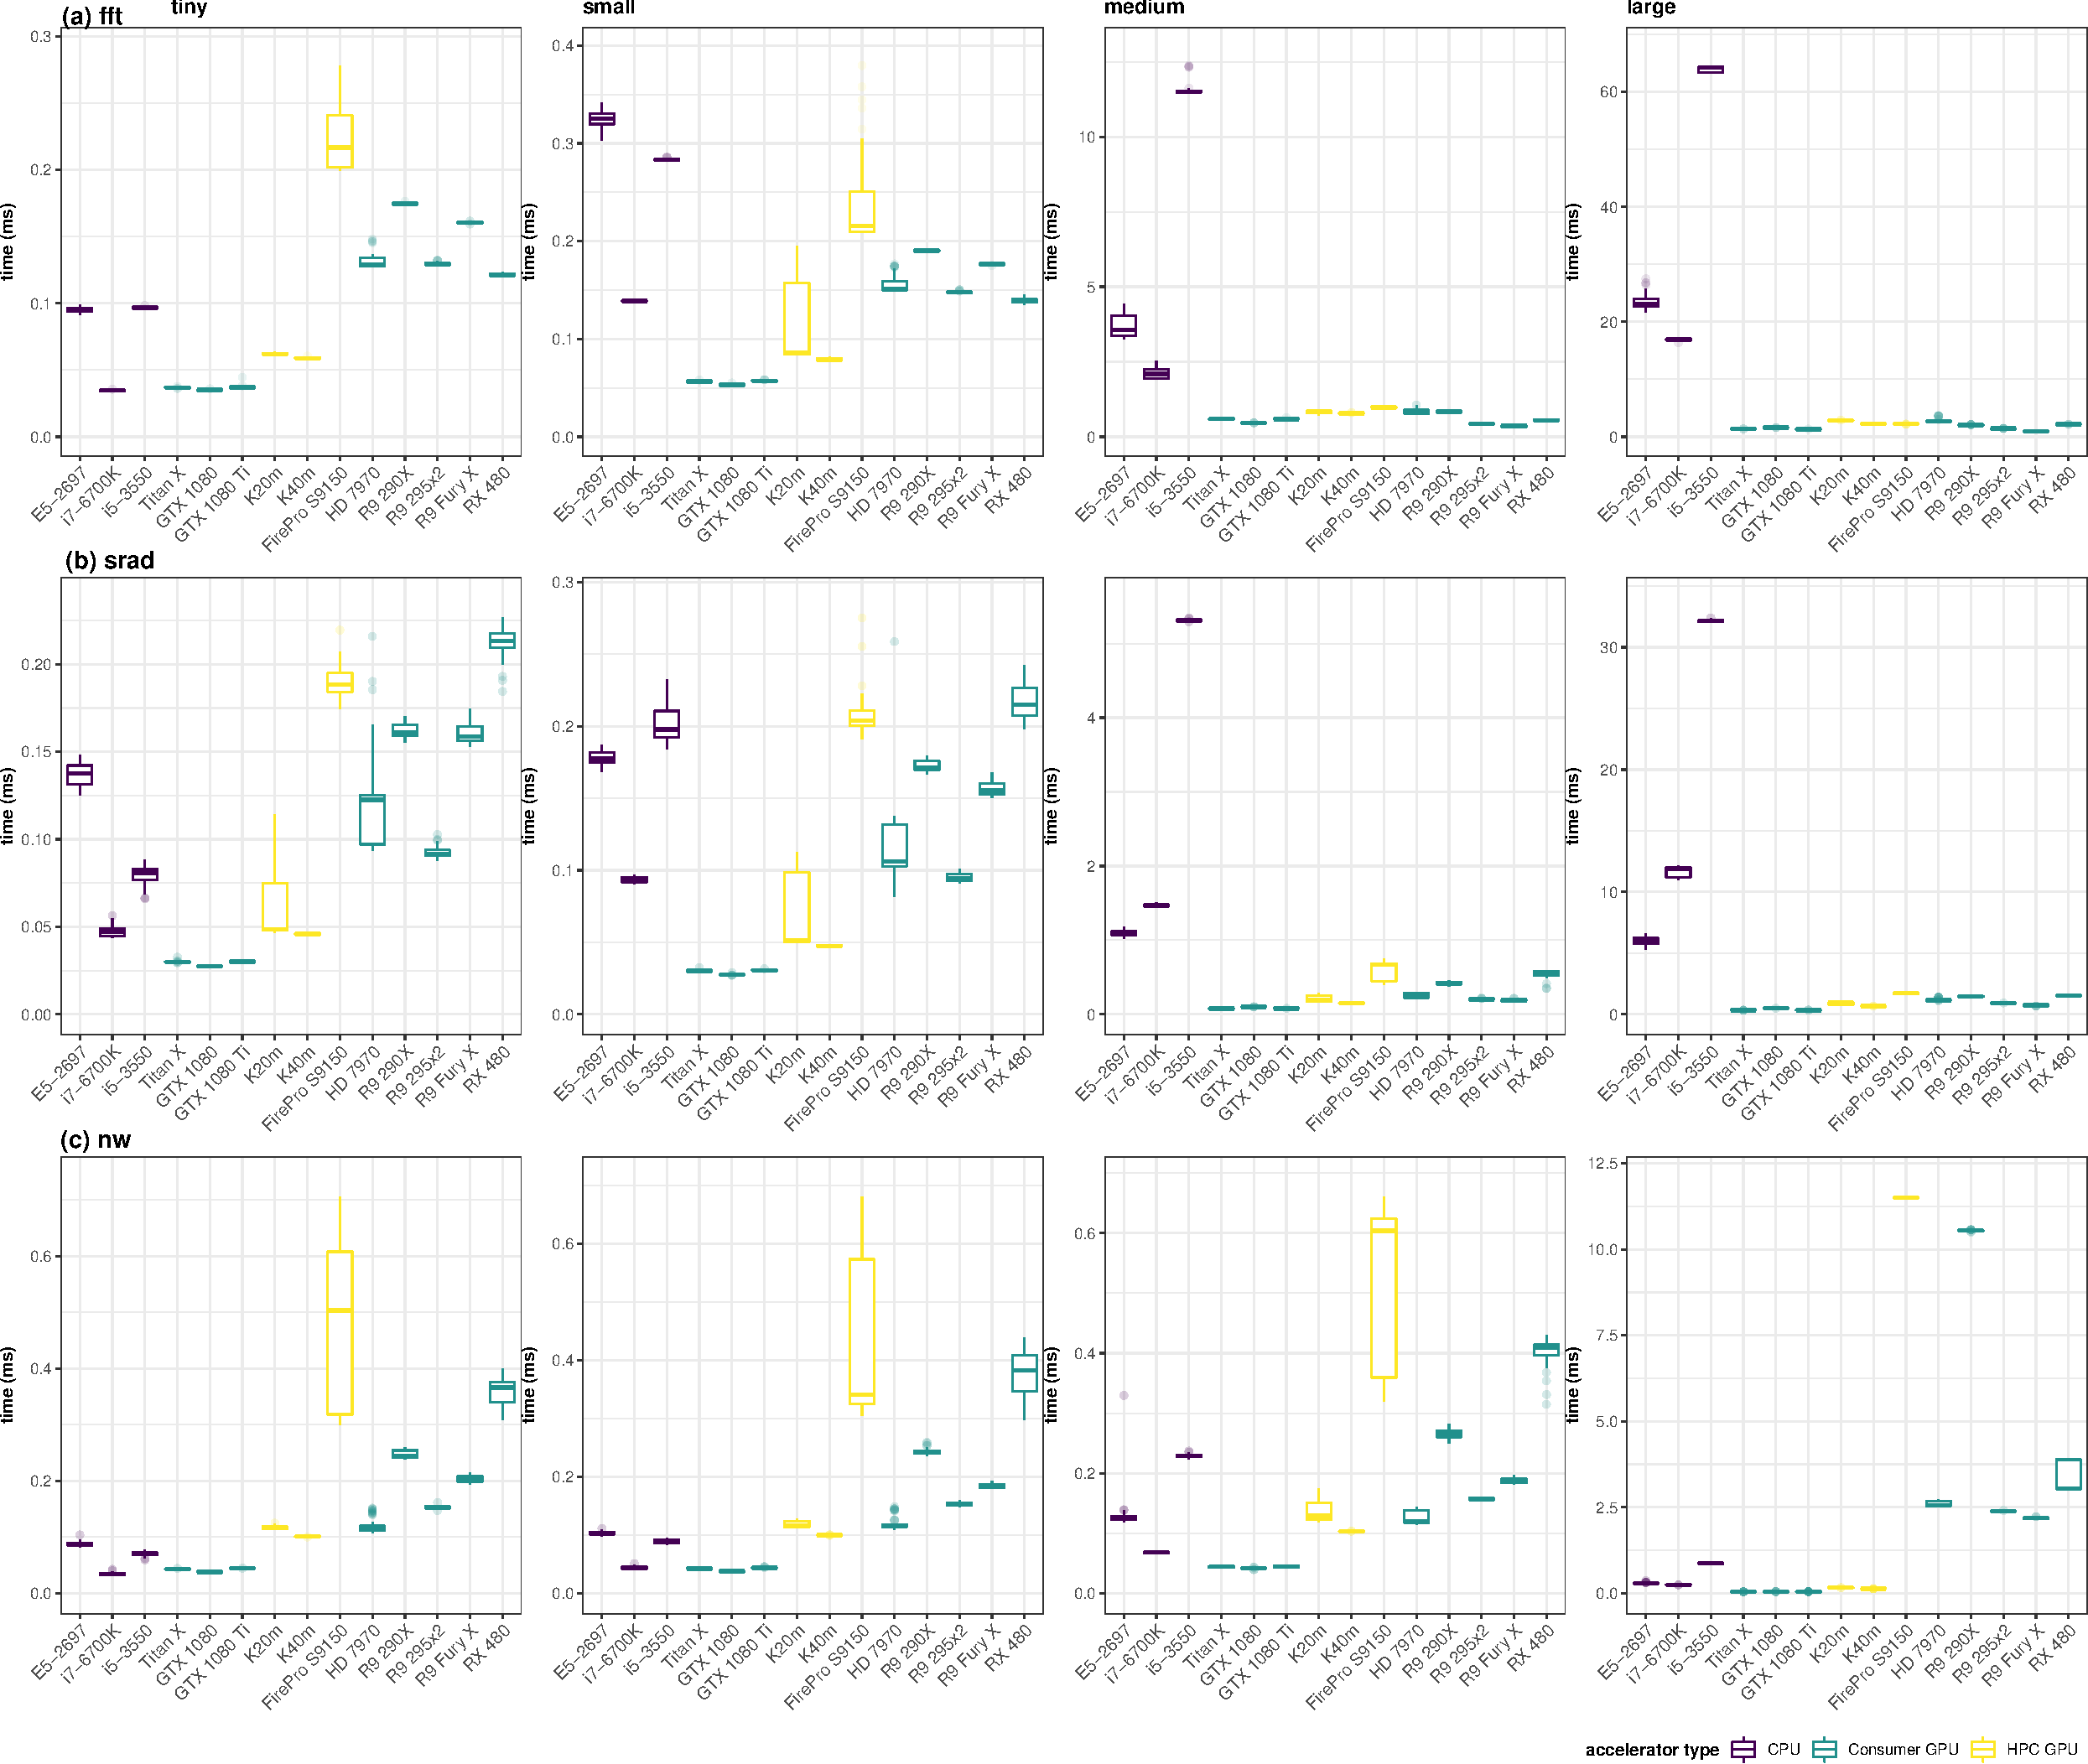
\includegraphics[width=\textwidth,keepaspectratio]{figures/new-time-results/generate_main_4x2_bandwplot}
    \caption{Benchmark kernel execution times on different hardware platforms (continued)}
    \label{fig:time2}
\end{figure*}

\begin{figure*}
    \centering
    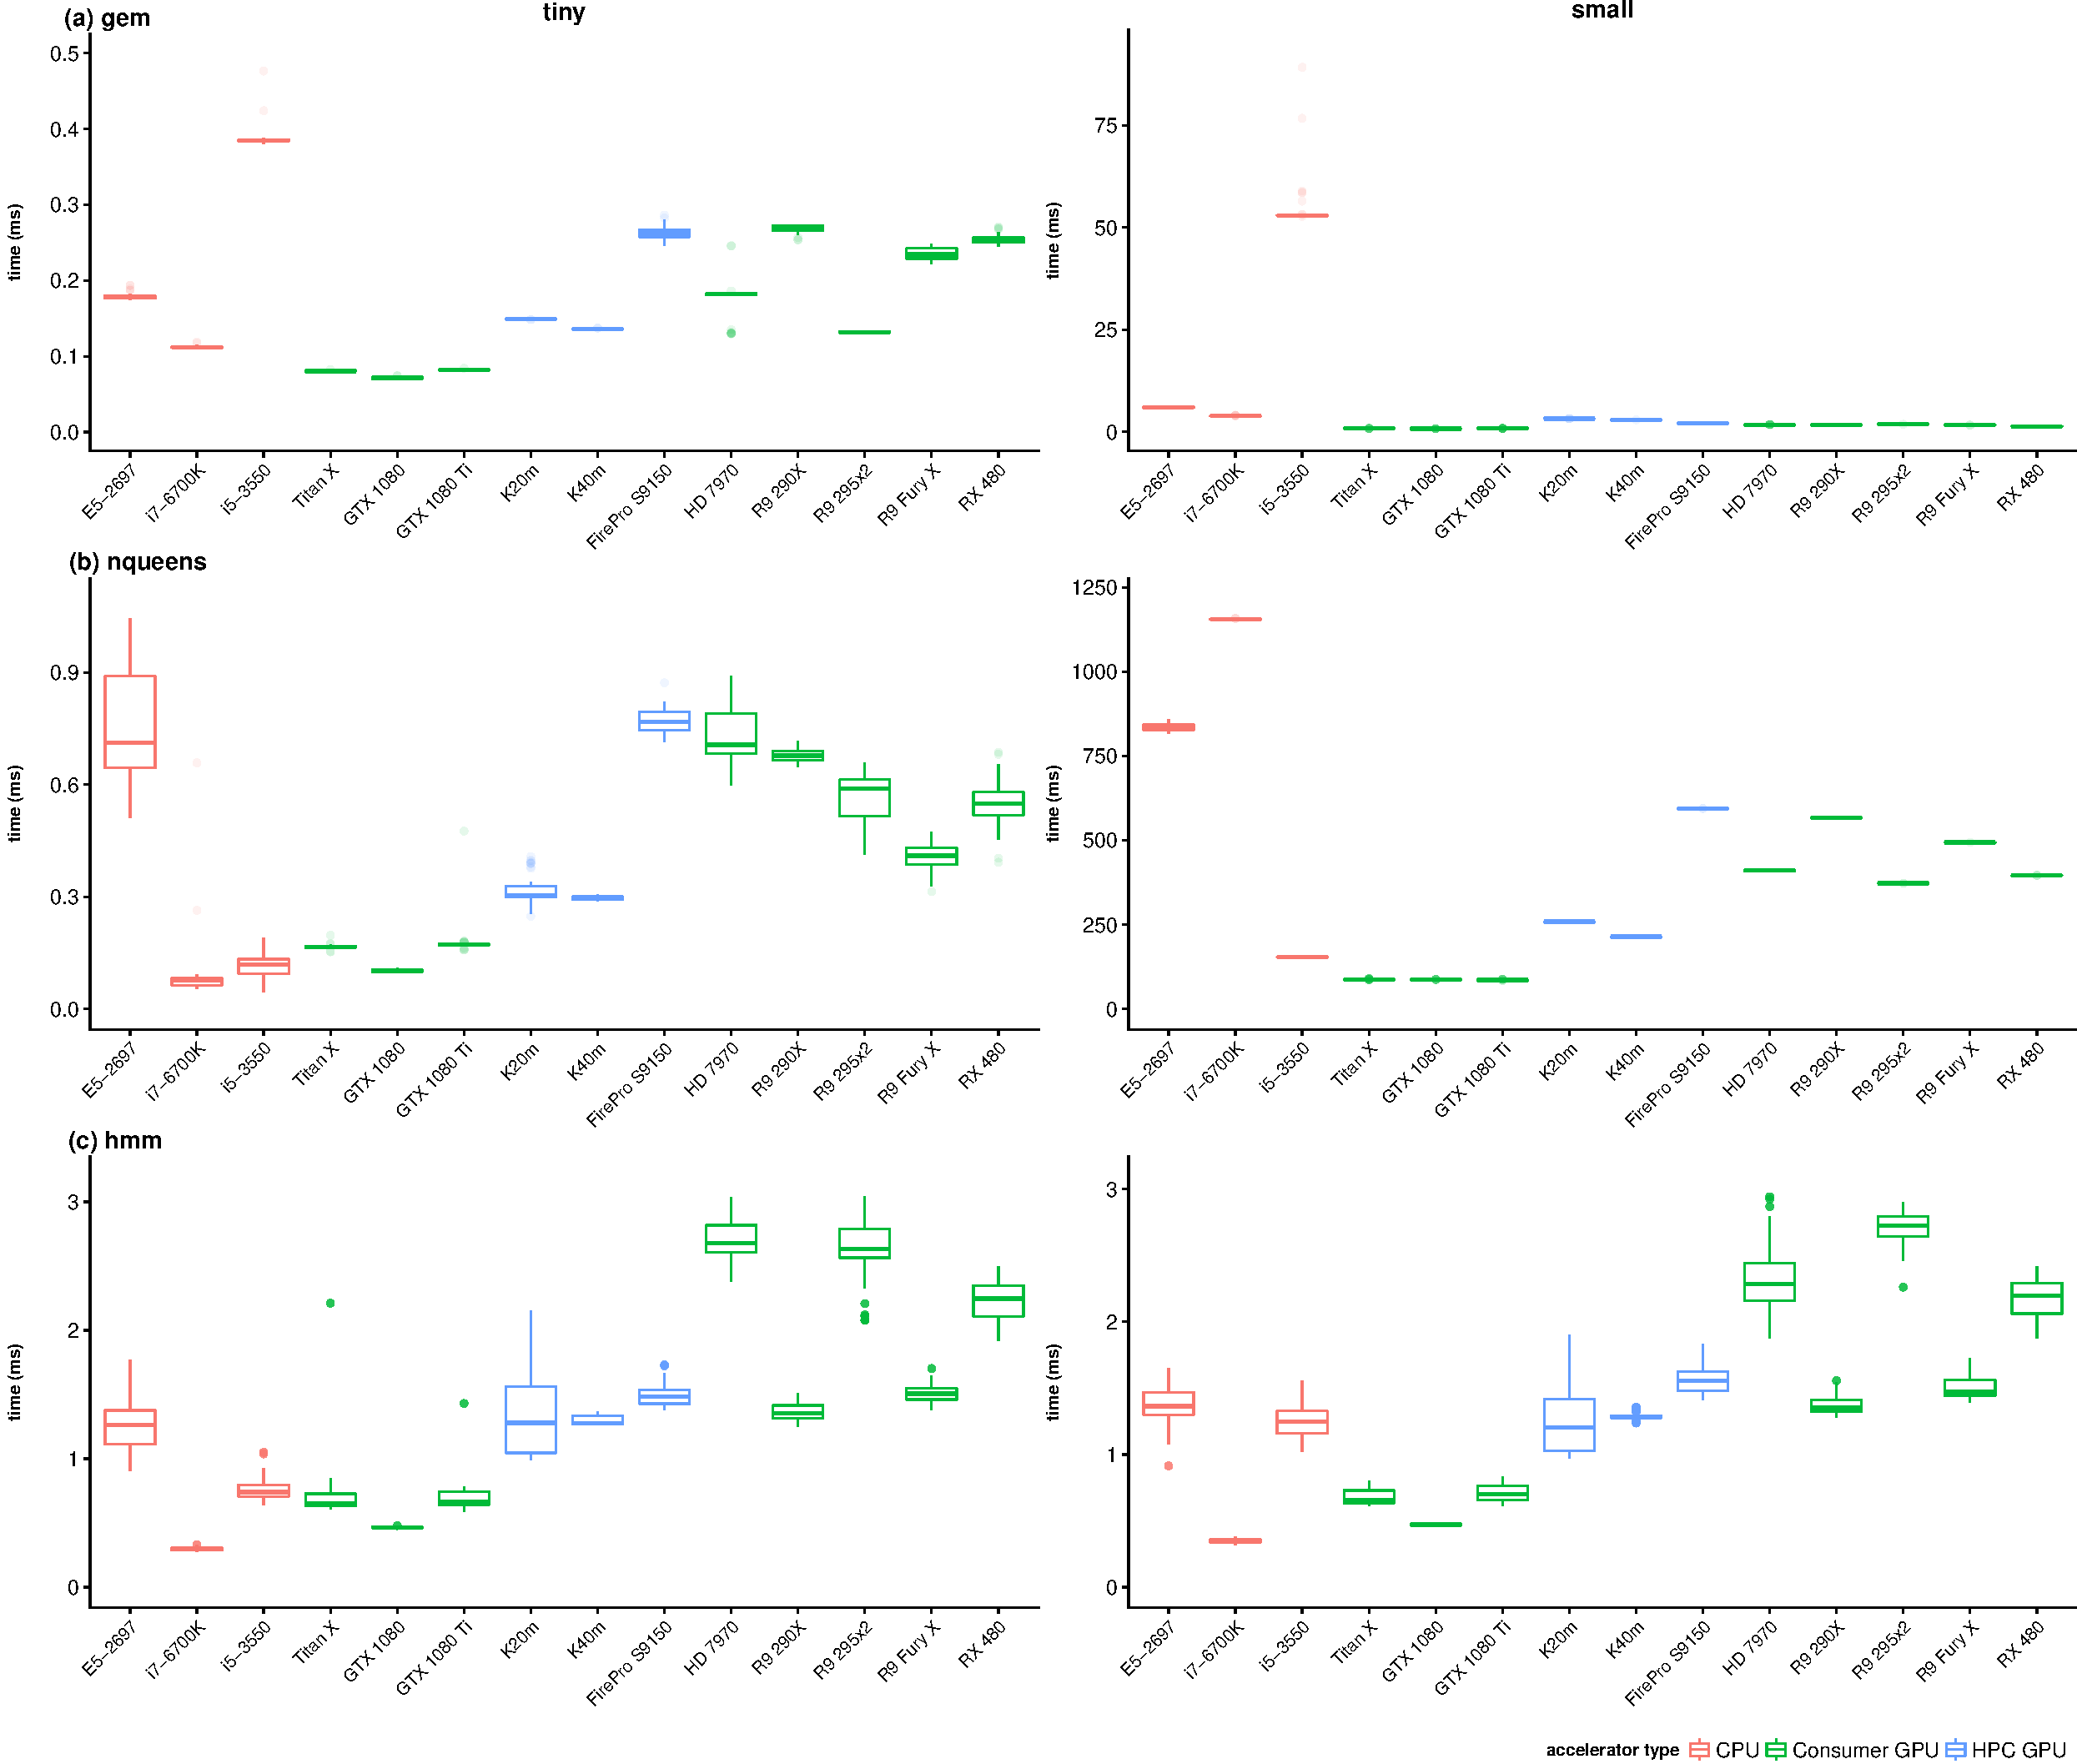
\includegraphics[width=\textwidth,keepaspectratio]{figures/new-time-results/generate_main_2x3_bandwplot}
    \caption{Single problem sized benchmarks of kernel execution times on different hardware platforms}
    \label{fig:time3}
\end{figure*}


Examining the transition from tiny to large problem sizes (from left to right) in Figure~\ref{fig:time2}a shows the performance gap between CPU and GPU architectures widening for {\tt srad} -- indicating codes representative of structured grid dwarfs are well suited to GPUs.

In contrast, Figure~\ref{fig:time2}b shows Dynamic Programming problems have performance results tied to micro-architecture or OpenCL runtime support and can not be explained solely by considering accelerator type.
For instance, the Intel CPUs and NVIDIA GPUs perform comparably over all problem sizes, whereas all AMD GPUs exhibit worse performance as size increases.

For most benchmarks, the coefficient of variation in execution times is much greater for devices with a lower clock frequency, regardless of accelerator type.
While execution time increases with problem size for all benchmarks and platforms, the modern GPUs (Titan X, GTX1080, GTX1080Ti, R9 Fury X and RX 480) performed relatively better for large problem sizes, possibly due to their greater second-level cache size compared to the other platforms.
A notable exception is {\tt k-means} for which CPU execution times were comparable to GPU, which reflects the relatively low ratio of floating-point to memory operations in the benchmark.

Generally, the HPC GPUs are older and were designed to alleviate global memory limitations amongst consumer GPUs of the time.
(Global memory size is not listed in Table~\ref{tab:hardware}.)
Despite their larger memory sizes, the clock speed of all HPC GPUs is slower than all evaluated consumer GPUs.
While the HPC GPUs (devices 7-9, in yellow) outperformed consumer GPUs of the same generation (devices 10-13, in green) for most benchmarks and problem sizes, they were always beaten by more modern GPUs.
This is no surprise since all selected problem sizes fit within the global memory of all devices.

A comparison between CPUs (devices 1-3, in purple) indicates the importance of examining multiple problem sizes.
Medium-sized problems were designed to fit within the L3 cache of the i7-6700K system, and this conveniently also fits within the L3 cache of the Xeon E5-2697 v2.
However, the older i5-3550 CPU has a smaller L3 cache and exhibits worse performance when moving from small to medium problem sizes, and is shown in Figures~\ref{fig:time}b,~\ref{fig:time}d,~\ref{fig:time}e and ~\ref{fig:time2}a,

Increasing problem size also hinders the performance in certain circumstances for GPU devices.
For example, Figure~\ref{fig:time2}b shows a widening performance gap over each increase in problem size between AMD GPUs and the other devices.

Predicted application properties for the various Berkeley Dwarfs are evident in the measured runtime results.
For example, Asanovi\'{c} et al.~\cite{asanovic2006landscape} state that applications from the Spectral Methods dwarf is memory latency limited.
If we examine {\tt dwt} and {\tt fft} -- the applications which represent Spectral Methods -- in Figure~\ref{fig:time}d and Figure~\ref{fig:time}e respectively, we see that for medium problem sizes the execution times match the higher memory latency of the L3 cache of CPU devices relative to the GPU counterparts.
The trend only increases with problem size: the large size shows the CPU devices frequently accessing main memory while the GPUs' larger memory ensures a lower memory access latency.
\todo{What is the memory size for the GPUs, and what is the difference in latency?}
It is expected if had we extended this study to an even larger problem size that would not fit on GPU global memory, much higher performance penalties would be experienced over GPU devices, since the PCI-E interconnect has a higher latency than a memory access to main memory from the CPU systems.
As a further example, Asanovi\'{c} et al.~\cite{asanovic2006landscape} state that the Structured Grid dwarf is memory bandwidth limited.
The Structured Grid dwarf is represented by the {\tt srad} benchmark shown in Figure~\ref{fig:time2}a.
GPUs exhibit lower execution times than CPUs, which would be expected in a memory bandwidth-limited code as GPU devices offer higher bandwidth than a system interconnect.

\todo[inline]{The remaining applications could be examined in terms of dwarf}

\end{document}
